\chapter{Technical Analysis}

\section{Event Analysis and Review}

The FreeStyle Libre sensor takes readings every 60 seconds, but it does not retain all of these, because of what we presume are storage limitations. Instead, it keeps half an hour of high definition data (30 values separated by 60 seconds) and an additional 7.5 hrs of coarse 15 minute data (45 values separated 15 min), disregarding the rest. The sensor also contains a power source, for both the electronics and the measurement mechanism, and a thermometer. When scanned, the sensor provides the stored data (30min fine, 7.5hr coarse), associated internal time, and uncalibrated temperature information. This information was gained during data analysis, as discussed later.

The sensor provides a series of raw, unsmoothed datapoints at a lag from ground truth, which the reader aims to transform into clinically useful information. Their precise algorithm is appropriately a trade secret, but provides transformed historical data, point estimate, and trend. Sometimes it will refuse to display any data, typically if glucose levels are changing very rapidly. Since the company provided accuracy study uses industry-standard Yellow Springs Instrument levels as ground truth, the provided data can safely be assumed to be intended to represent venous blood glucose. Their user manual also provides a chart for interpreting the glucose trend arrow, as shown in Figure~\ref{fig:arrows}\footnote{from the FreeStyle Libre manual supplied with the sensor.}. 

We found that the reader point estimate provides greater mathematical accuracy to blood glucose than the associated raw sensor value. The historical trend line is displayed in too low a resolution for much accuracy discussion, but as discussed later, more accurate data can be gained. The trend arrow will be discussed more in depth in future. Of course, clinical accuracy must also be considered.

\begin{figure}[ht]
\centering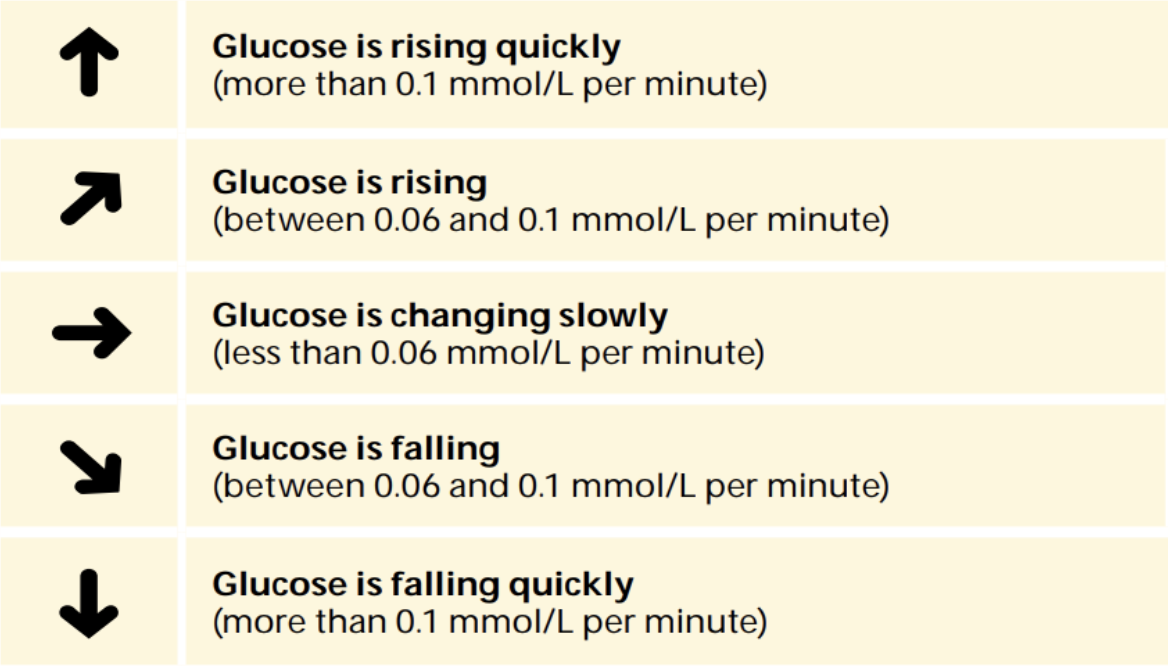
\includegraphics[width=1.0\linewidth]{images/arrows.png}
\caption{Conditions where arrows are displayed.}
\label{fig:arrows}
\end{figure}

As well as processing and displaying the raw data, the reader provides several extra capabilities. It allows users to set date, time and target glucose range. With each scan, it also allows the user to add flags to record extra events such as insulin, food, medication and exercise. Flags for other events can be added using the software. Historical records can be viewed as well as limited analytics such as weekly averages, time in range, and typical daily trend. The reader can also act as an independent blood glucose or ketone meter.  

\section{Sensor Chemistry}

The technology underlying most commercially available continuous glucose monitors is the same. They are inserted subcutaneously, typically into the arm or stomach. They consist of an implanted, flexible catheter connected to the external plastic shell, which is typically attached to the skin with adhesive. The catheter acts as an amperometric biosensor and takes a raw measurement of interstitial glucose. The external hardware provides power, keeps time, records the measurements, and is sometimes attached to an optional transmitter. Currently, there are three main commercial brands; DexCom, Medtronic, and Abbott.

\subsection{Amperometric Glucose Biosensors}

An amperometric glucose biosensor uses redox electrodes to create and measure a current proportional to interstitial glucose concentration. From the current, they can closely estimate the actual glucose concentration. If there’s too much noise for the current and concentration to have a constant ratio, the device will require regular recalibration by matching with blood glucose tests. Since most CGMs aim to eliminate the need for BGMs, manufactures aim to reduce noise, while maintaining sensor lifespan and comfort.

\begin{figure}[ht]
\centering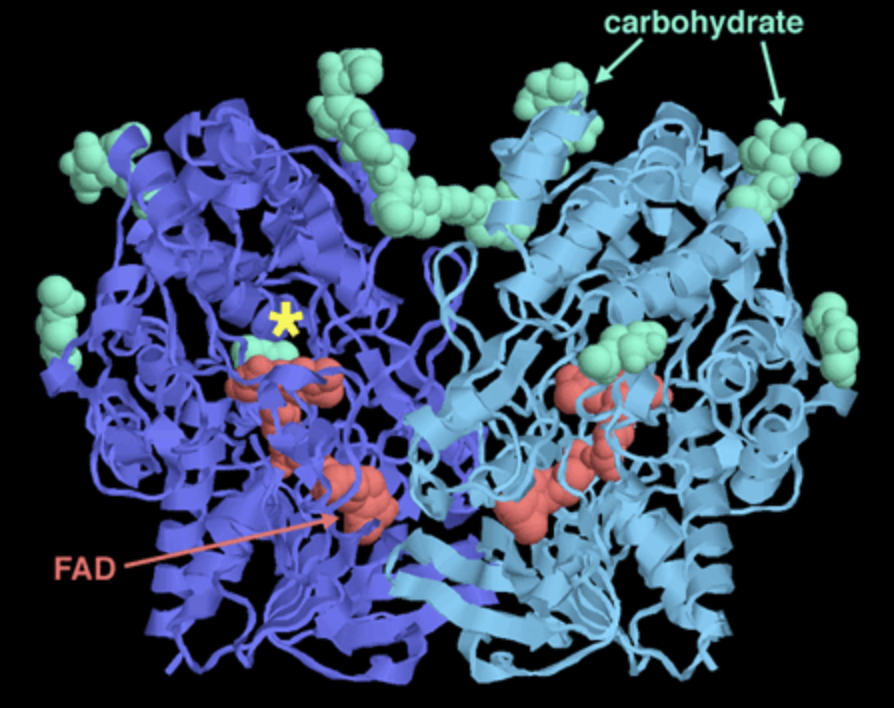
\includegraphics[width=1.0\linewidth]{images/mom.png}
\caption{Location of flavin adenine dinucleotide (FAD) co-factor in glucose oxidase.}
\label{fig:mom}
\end{figure}

In order to produce the proportional current, an amperometric biosensor electro-oxidizes glucose with the  flavin adenine dinucleotide (FAD) co-factor of glucose oxidase as shown in Equation~\ref{eq:one}, then measures the current provided when re-oxidizing the reduced glucose oxidase. It is difficult to directly oxidize the FAD co-factor, since it’s buried deep within the molecule (Figure~\ref{fig:mom}), so a mediator is used. This creates a three step system: oxidize glucose with glucose oxidase, react with the mediator, then oxidize the reduced mediator. At each of these steps, the concentration of the products remains proportional to the concentration of glucose. At the last step, the electro-oxidation of the mediator, the current produced will also be proportional. The speed of electron movement will be proportional to the reaction rate, which will be proportional to the reactant (reduced mediator) concentration\cite{noauthor_amperometric_nodate}. This provides an acceptable raw representation for interstitial fluid glucose concentration. Anything that interferes with any of these proportions creates noise.

Most often, oxygen is used for the mediator. This results in the chain of reactions shown in Equations~\ref{eq:two} and \ref{eq:three}. Oxygen is a useful mediator, because instead of needing to be immobilized in on the electrode, it can be taken in vivo. However, the reactions need a higher ratio of oxygen to glucose that is found in interstitial fluid to be successful. To overcome this, both Dexcom and Medtronic have developed complicated membranes that only allow the desired ratios in - remaining, of course, in proportion to the global body glucose\cite{noauthor_mary_nodate}. However, this introduces more noise. The heavy design requirements for the membrane also mean that it lacks flexibility to control other noise-inducing factors. This contributes to both those systems requiring twice-daily calibration.

\begin{equation} \label{eq:one}
FAD-GO_x + glucose \rightarrow FADH_2-GO_x + gluconolactone
\end{equation}

Reduction half-equation: $FAD-GO_x + 2H_+ + 2e+-  FADH_2-GO_x$\\ 
Oxidation half-equation: $glucose \rightarrow gluconolactone + 2H_+ + 2e_- $

\begin{equation} \label{eq:two}
FADH_2 - GO_x + O_2 \rightarrow H_2O_2 + FAD-GO_x 
\end{equation}

Reduction half-equation: $O_2 + 2H_+ + 2e_- \rightarrow H_2O_2$ \\
Oxidation half-equation: $FADH_2 \rightarrow FAD-GO_x + 2H_+ + 2e_-$ 

\begin{equation} \label{eq:three}
 H_2O_2 \rightarrow O_2 + 2H_+ + 2e_- 
\end{equation}

Abbott overcame this issue with their trademarked Wired Enzyme technology\cite{noauthor_sensor_nodate}. This uses immobilized osmium complexes as their mediator, resulting in the reactions shown in Equation~\ref{eq:four}. This has several benefits. It avoids involving several confounding variables into the equation by removing the need to use internal oxygen and by oxidizing the glucose oxidase in place, instead of in solution. Most usefully, re-oxidizing the osmium requires a much lower voltage than doing so for the oxygen. This avoids interference from other substances, like uric acid or medical acetaminophen\cite{noauthor_mary_nodate}. Overall, the Wired Enzyme decreases noise enough that it need only be calibrated in the factory, since the current to glucose concentration ratio stays constant\cite{hoss_feasibility_2014}. On the other hand, it means that Abbott devices have a clear expiration date, since they become completely unusable once they run out of osmium.

\begin{equation} \label{eq:four}
FADH_2 - GO_x + 2Os_{3+} \rightarrow  2Os_{2+} + FAD-GO_x + 2H_+ 
\end{equation}
Reduction half-equation: $2Os_{3+} + 2e_- \rightarrow 2Os_{2+}$\\ 
Oxidation half-equation: $FADH_2 \rightarrow FAD-GO_x + 2H_+ + 2e_-$ 

Other factors also confound accuracy. Regardless of what mediator a sensor uses, it has to resolve biofouling. Tissue response to a foreign body injection can mean that local glucose stops accurately representing global glucose. Companies increasingly minimize this with improving biocompatible material technology. Another problem which is yet to be properly solved is tissue inflammation upon injection. This typically means that initial results will be less accurate, getting more so as the inflammation goes down.

One environmental variable that hasn’t been properly addressed is temperature. All amperometric biosensors rely on enzyme reactions, which vary heavily with temperature\cite{noauthor_accuracy_nodate}. Enzyme activity increases alongside temperature, which carries over throughout the process and hence to the reported glucose values. No mention can be found of how any CGM controls for this within the sensor hardware, and it’s difficult to imagine how they could. No mention was found of whether this was controlled for in software, and anecdotal evidence suggests that the current methods are ineffective.

CGM sensors record interstitial fluid glucose by using an amperometric biosensor to measure a current that’s directly proportional to glucose concentration. In order to make sure that the proportionality remains, companies have put a lot of work into minimizing chemical and biological interference. 

